\chapter{Multimodal Inference of Mind SCAIN}
\par
本論文では,行動情報と発話情報の両方を活用する心的状態推定システムMultimodal Inference of Mind SCAIN (MIoM SCAIN)を提案する.MIoM SCAINは,人間の信念や行動,発話および人間が存在する環境の状態を基に心的状態を推定する.行動情報と発話情報の両方を心的状態の推定に活用することで,発話による行動の解釈の変化や行動による発話の解釈の変化を捉え,行動情報と発話情報の相互作用を考慮して心的状態を推定する.

\par
MIoM SCAINは,環境の状態や人間の心的状態を部分的に観測可能なマルコフ決定過程として表す.また,心的状態の推定値はそれぞれの候補に対し尤度が与えられたパーティクルフィルタとして表され,心的状態を一意に決定するのではなく同時に複数保持し,時刻が経過する度に各パーティクルの尤度を更新していく.各時刻における人間の信念や行動,発話および人間が存在する環境の状態をベイズ推論に適用し,環境中で人間が観測できていない部分についての信念と欲求を逐次的に推定する.


\section{アルゴリズム}

\par
MIoM SCAINにおける推定処理の流れをを図\ref{fig:sys_arc}に示す.
\begin{figure}[htbp]
  \begin{center}
    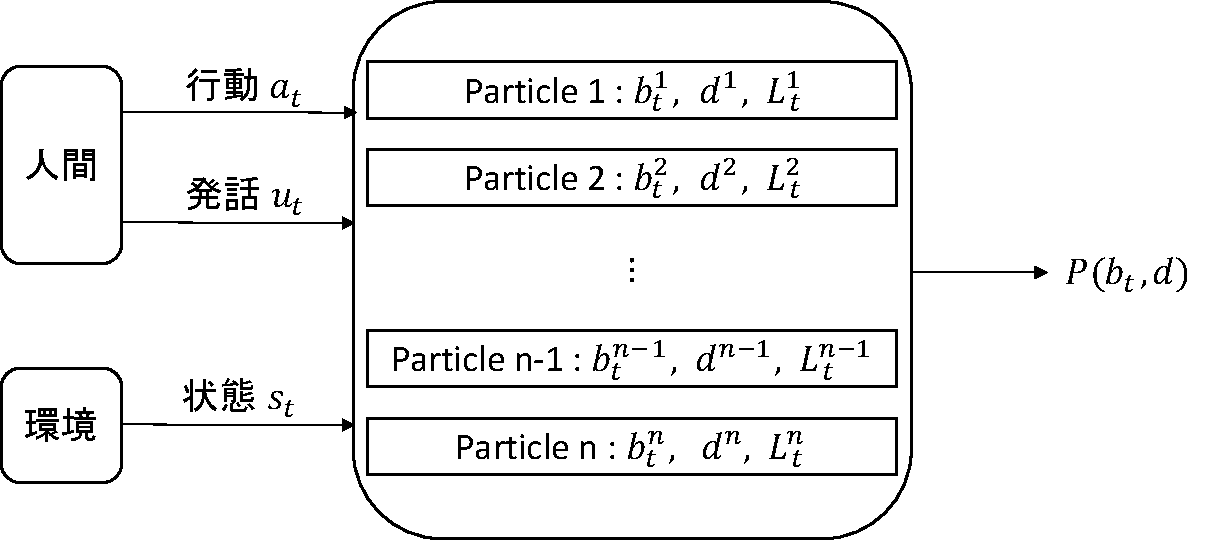
\includegraphics[scale=0.75]{./bt1.pdf}
    \caption{MIoM SCAINによる推定処理}
    \label{fig:sys_arc}
  \end{center}
\end{figure}
図\ref{fig:sys_arc}に示すように,MIoM SCAINは時刻$t$における人間の行動$a_t$,発話$u_t$および環境の状態$s_t$から信念と欲求の確率を出力する.MIoM SCAINは信念$b_t$と欲求$d$の組み合わせとその尤度$L$を持つパーティクルフィルタとして表現され,$a_t,u_t,s_t$と$k$番目のパーティクルが持つ信念$b_t^k$と欲求$d^k$を基に尤度$L^k$が更新される.ここで,尤度$L^k$は次のように表すことができる.
\begin{equation}
  \begin{split}
  \label{pf}
  L^k=P(b_t^k,d^k|s_{1:t},a_{1:t-1},u_{1:t-1})
  \end{split}
\end{equation}
ここで,$u_{1:t-1}$は,時刻$1$から時刻$t-1$までの人間の発話履歴,$P(b_t,d|s_{1:t},a_{1:t-1},u_{1:t-1})$は,$s_{1:t},a_{1:t-1}およびu_{1:t-1}$から計算される$b_t$と$d$の確率である.

\par
図\ref{fig:miom}にMIoM SCAINにおけるベイズ推論の様子を示す.
\begin{figure}[htbp]
  \begin{center}
    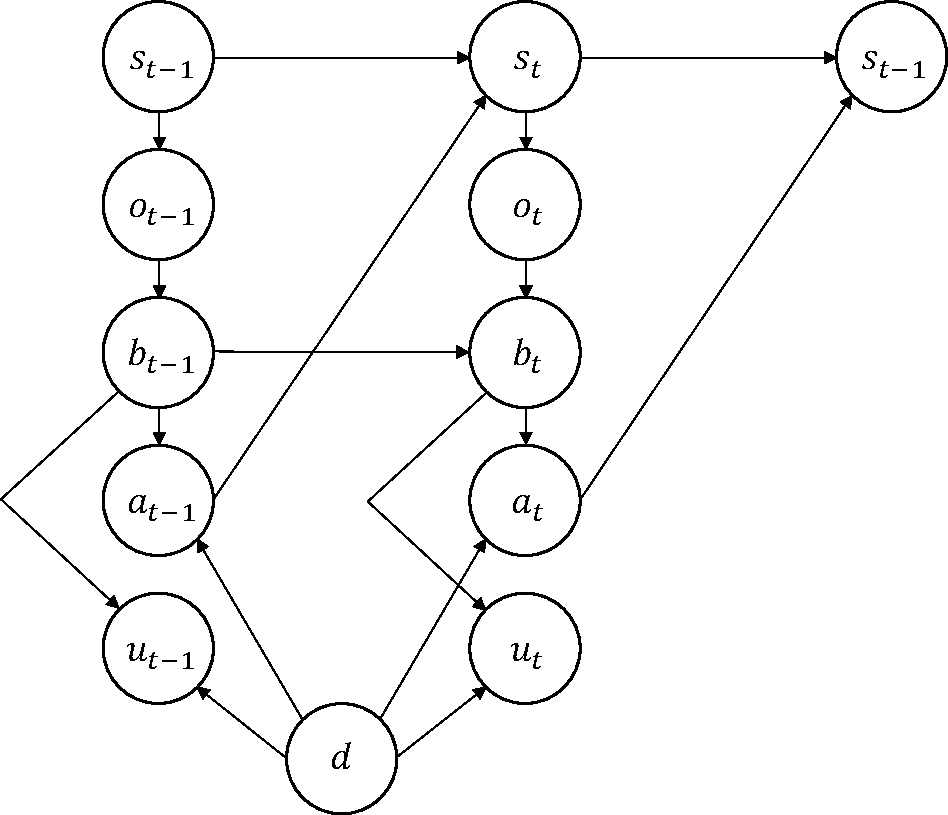
\includegraphics[scale=0.75]{./miom.pdf}
    \caption{MIoM SCAINにおけるベイズ推定}
    \label{fig:miom}
  \end{center}
\end{figure}
MIoM SCAINにおけるベイズ推論では,BToMと同様に時刻$t$における環境の状態$s_{t}$を基に人間の観測状況$o_{t}$が決まる.また,$o_{t}$を基に人間の信念$b_{t}$が決まり,$b_{t}$と人間の欲求$d$から人間の行動$a_{t}$が決まる.それに加え,MIoM SCAINでは$b_t$と$d$から人間の発話$u_t$が決まる.また$a_{t}$が起こることにより,環境の状態は$s_{t+1}$に変化し,人間の観測状況,信念,行動および発話が再び計算される.MIoM SCAINでは各パーティクルの尤度である式(\ref{pf})を計算することを目的としている.以下に,式(\ref{pf})にベイズの定理を適用した過程を示す.

\begin{equation}
  \begin{split}
  \label{eq_miom}
  L^k&=P(b_t^k,d^k|s_{1:t},a_{1:t-1},u_{1:t-1})\\
  &\propto P(b_t^k,d^k,s_{1:t},a_{1:t-1},u_{1:t-1})\\
  &= \sum_{b_{t-1}^k,o_t}P(b_t^k,d^k,s_{1:t},a_{1:t-1},u_{1:t-1},b_{t-1}^k,o_t)\\
  &= \sum_{b_{t-1}^k,o_t}P(b_t^k|d^k,s_{1:t},a_{1:t-1},u_{1:t-1},b_{t-1}^k,o_t)\cdot P(d^k,s_{1:t},a_{1:t-1},u_{1:t-1},b_{t-1}^k,o_t)\\
  &= \sum_{b_{t-1}^k,o_t}P(b_t^k|b_{t-1}^k,o_t)\cdot P(o_t|d^k,s_{1:t},a_{1:t-1},u_{1:t-1},b_{t-1}^k)\\
  &\hspace{5cm} \cdot P(d^k,s_{1:t},a_{1:t-1},u_{1:t-1},b_{t-1}^k)\\
  &= \sum_{b_{t-1}^k,o_t}P(b_t^k|b_{t-1}^k,o_t)\cdot P(o_t|s_t)\cdot P(s_t|s_{t-1},a_{t-1})\\
  &\hspace{3cm} \cdot P(a_{t-1}|b_{t-1}^k,d^k)\cdot P(u_{t-1}|b_{t-1}^k,d^k)\cdot P(b_{t-1}^k,d^k,s_{t-1},a_{t-2},u_{t-2})\\
  \end{split}
\end{equation}


ここで,$P(b_t^k|b_{t-1}^k,o_t)$は人間の観測$o_t$によって$k$番目のパーティクルの信念$b_t^k$が更新される確率,$P(o_t|s_t)$は環境の状態$s_t$において人間が観測状況$o_t$を得る確率,$P(s_t|s_{t-1},a_{t-1})$は環境の状態$s_{t-1}$において人間が行動$a_{t-1}$を起こした時に環境の状態が$s_{t}$になる確率,$P(a_{t-1}|b_{t-1}^k,d^k)$は$k$番目のパーティクルが信念$b_{t-1}^k$,欲求$d^k$を持っている時に行動$a_{t-1}$を起こす確率,$P(u_{t-1}|b_{t-1}^k,d^k)$は$k$番目のパーティクルが信念$b_{t-1}^k$,欲求$d^k$を持っている時に発話$u_t$を起こす確率,$P(b_{t-1}^k,d^k,s_{t-1},a_{t-2},u_{t-2})$は時刻$t-1$における$k$番目のパーティクルの尤度である.式(\ref{eq_miom})より,$L^k$は初期値$P(b_1,d,s_1,a_0,u_0)$を決めて順次更新する計算により求めることができる.また,$L^k$は$P(b_t^k|b_{t-1}^k,o_t)$,$P(o_t|s_t)$,$P(s_t|s_{t-1},a_{t-1})$,$P(a_{t-1}|b_{t-1}^k,d^k)$および$(u_{t-1}|b_{t-1}^k,d^k)$の乗算として表すことができる.

\section{実装}
% それぞれの生起確率がどのように計算されるかを記載
MIoM SCAINでは,各時刻における$P(b_t^k|b_{t-1}^k,o_t)$,$P(o_t|s_t)$,$P(s_t|s_{t-1},a_{t-1})$,$P(a_{t-1}|b_{t-1}^k,d^k)$および$P(u_{t-1}|b_{t-1}^k,d^k)$を計算し乗算したものを足し合わせることで,その時刻における信念と欲求の尤度を計算する.$P(b_t^k|b_{t-1}^k,o_t)$は既に人間が$b_t^k$を観測しているかどうかを$o_t$と比較することにより計算する.
$P(a_{t-1}|b_{t-1}^k,d^k)$は信念$b_{t-1}^k$と欲求$d^k$を基に上,下,左,右の4方向の確率を計算する.$(u_{t-1}|b_{t-1}^k,d^k)$はWord2Vec\cite{mikolov2013efficient}により発話$u_t$を分散表現に変換した後,信念$b_{t-1}^k$と欲求$d^k$との類似度を基に計算する.
